\documentclass[aps,prl, notitlepage]{revtex4-1}
\usepackage{afterpage}
\usepackage{amssymb}
\usepackage{amsbsy}
\usepackage{amsmath}
\usepackage{graphicx}
\usepackage{dcolumn}
\usepackage{bm}
\usepackage{natbib}
\usepackage{epsfig}
\usepackage{epstopdf}
\usepackage{dsfont}

\usepackage{hyperref}
\usepackage[usenames,dvipsnames]{xcolor}
\definecolor{med-blue}{RGB}{25,25,112}
\hypersetup{colorlinks, linkcolor={red},citecolor={blue}, urlcolor={MidnightBlue}}

%%%%%%%%%% Prefix a "S" to all equations, figures, tables and reset the counter %%%%%%%%%%
\setcounter{equation}{0}
\setcounter{figure}{0}
\setcounter{table}{0}
\setcounter{page}{1}
\makeatletter
\renewcommand*{\theequation}{S\arabic{equation}}
\renewcommand*{\thefigure}{S\arabic{figure}}
\renewcommand*{\bibnumfmt}[1]{[r#1]}
\renewcommand*{\citenumfont}[1]{r#1}
%%%%%%%%%% Prefix a "S" to all equations, figures, tables and reset the counter %%%%%%%%%%
\begin{document}
\title{Supplementary Materials}
\maketitle
In these supplementary notes, we detail some of the methodologies used to obtain the results detailed in the main paper. Our starting point is the transformed Hamiltonian in Eq.~$(2)$ of the main paper \textit{viz.}
\begin{equation}
H(t) = - \alpha J \sum_{i}^{L}  J_i \left(c^{\dagger}_i c^{\dagger}_{i+1} + c^{\dagger}_i c_{i+1}  + {\rm h.c.}\right)
- 2 \sum_i^{L} \left\{h(t)+\alpha h_i\right\} c^{\dagger}_i c_i,
\label{H_Fermi:suppl}
\end{equation}
with $h(t)=h_0\sin{\omega t}$. The first section elaborates on the numerical methods used to gather the time-magnetization data from the Hamiltonian above. The second section details the Floquet-RG flow equations used to pinpoint the approximate unitary transformation needed to obtain the effective Hamiltonian $H_{\rm eff}$ in the main paper. The final section details comparison of numerical evolution of the $H_{\rm eff}$- dynamics with that of the full Hamiltonian, as well as key qualitative observations in the former observed in the latter.

\section{\sc Numerical Methodology:}
In order to numerically simulate the time-dynamics of the Hamiltonian in Eq.~\ref{H_Fermi:suppl}, we rewrite it in terms of free fermions~\cite{Lieb}. Though the transformation is non-local in nature, we exploit a natural ordering in the sites to yield a Hamiltonian identical to Eq.~\ref{H_Fermi:suppl} (except with free fermions instead of hard-sphere bosons)  by canceling out nonlocal contributions. The present disordered case can be block-diagonalized by rewriting Eq.~\ref{H_Fermi:suppl}, with free fermions, in terms of Nambu spinors $\Psi$:
\begin{eqnarray}
\label{eq:nambu}
{H}(t) &=& \Psi^\dagger \bar{H}(t) \Psi , \nonumber \\
\Psi^\dagger &\equiv& \begin{pmatrix}
                  c^\dagger_1 & c^\dagger_2 & \dots & c^\dagger_L,c^{\;}_1 & c^{\;}_2 & \dots & c^{\;}_L  
                 \end{pmatrix}, \nonumber \\
\bar{H}(t) &\equiv& \begin{pmatrix}
                A(t) & B(t) \\
                -B(t) & -A(t) 
               \end{pmatrix}.
\end{eqnarray}
Here, $A$ and $B$ are real $L\times L$ matrices. The matrix $A=A^d(t)+A^o$, where $A^d_{i,j}(t)=-\left[h(t)+\alpha h_i\right]\delta_{i,j}$ is diagonal. The non-zero elements of $A^o$ and $B(t)$ are given by $A^o_{i,i+1}=A^o_{i+1,i}=-\alpha J J_i /2$, $B_{i,i+1}(t)=-B_{i+1,i}(t)=-\alpha J J_i/2$. The Heisenberg equations of motion for the operator $c^{\;}_{i,H}(t)$ are
\begin{equation}
\label{eq:heisenberg}
i \frac{\mathrm{d}}{\mathrm{d} t}c^{\;}_{i,H}(t) = U^\dagger(t)\left[c_i,H(t)\right]U(t),
\end{equation}
where the subscript $H$ denotes operators in the Heisenberg picture, and  $U(t)$ is the time translation that solves the Schr\"odinger equation of the Hamiltonian in Eq.~\ref{H_Fermi:suppl}. Note that, for every operator $O(t)$ in the Schr\"odinger picture, the corresponding operator in the Heisenberg picture, $O_H(t)=U^\dagger(t) O(t) U(t)$. We now substitute the last of Eq.~\ref{eq:nambu} into the rhs of Eq.~\ref{eq:heisenberg} to yield
\begin{equation}
\label{eq:dyn}
i \frac{\mathrm{d}}{\mathrm{d} t}c^{\;}_{i,H}(t) =  2\sum_j \bigg[A_{ij}(t)c^{\;}_{j,H}(t)+ B_{ij}(t)c^{\dagger}_{i,H}(t)\bigg].
\end{equation}
These equations can be solved by the trial solution $c^{\;}_{i,H}(t) = \sum_\mu \left[u_{i\mu}(t)\gamma_{\mu,H}(t)+v^\ast_{i\mu}(t)\gamma^\dagger_{\mu,H}(t)\right]$, where the Bogoliubov ansatz makes the many body state $|\Psi(t)\rangle$ the emergent vacuum of the modes  created by $\gamma^\dagger_{\mu}(t)$ $\forall t$ \textit{viz.} $|\Psi(t)\rangle \sim \prod_\mu \gamma_\mu(t) |0\rangle$, where the normalization has been suppressed, and the product is over all lattice sites. A necessary and sufficient condition for the emergent modes to generate the emergent vacuum is that $\gamma_\nu(t)|\Psi(t)\rangle = 0$, leading to  $ {d\over dt} \left( \gamma_\nu(t)|\Psi(t)\rangle \right) = 0$. In the Heisenberg picture, this condition can be rewritten as $i{d\over dt}\gamma_{\mu,H}(t)=0$. Using this result, we substitute the trial solution into Eq.~\ref{eq:dyn} and compare operator coefficients. This leads to the following dynamical system:
\begin{eqnarray} 
\label{BdG_tdep:eqn}
i\frac{d}{dt}u_{i\mu}(t) &=&  {2} \sum_{j=1}^{L} \bigg[A_{i,j}(t)u_{j\mu}(t)+ B_{i,j}(t)v_{j\mu}(t) \bigg] \nonumber \\
i\frac{d}{dt}v_{i\mu}(t) &=& -{2}\sum_{j=1}^{L} \bigg[A_{i,j}(t)v_{j\mu}(t)+ B_{i,j}(t)u_{j\mu}(t) \bigg].\nonumber \\
\end{eqnarray}
The objects $u_{j\mu}(t)$, $v_{j\mu}(t)$ can be encapsulated into $L\times L$ matrices $u(t)$ and $v(t)$. Unitary evolution and canonicality demands that $\{\gamma_\mu(t),\gamma^\dagger_\nu(t)\}=\delta_{\mu\nu},\{\gamma_\mu(t),\gamma_\nu(t)\}=\{\gamma^\dagger_\mu(t),\gamma^\dagger_\nu(t)\}=0$. Thus, $u^\dagger(t) u(t) + v^\dagger(t) v(t) = \mathds{1}$, and $v^T(t)u(t)+u^T(t)v(t) = 0$.  Any initial condition we choose must satisfy these conditions at $t=0$. Our choice of initial condition \textit{viz.} the classical ground state strongly polarized in the $+z$-direction, translates to $|\Psi(0)\rangle \sim \prod_i c^\dagger_i |0\rangle$. This can be set by putting $u(0)=0$, $v(0)=\mathds{1}$.

The magnetization per site can be shown via Jordan-Wigner transformation to be $\langle m^z(t)\rangle\equiv -1 + {2 \over L}\sum_i \langle \Psi(0) | c^\dagger_{i,H} (t)$ $c_{i,H}(t) |\Psi(0)\rangle$. Substituting the trial solution and using the canonical anti-commutation relations of $\gamma_\mu(t)$ simplifies the magnetization to 
\begin{equation}
 \label{eq:mag}
\langle m^z(t)\rangle = -1+\frac{2}{L} \; {\rm Tr}\left[ {v}^\dagger(t) {v}(t)\right].
\end{equation}
\noindent
The following exponential form fits the exact numerical data for the disorder-averaged magnetization very well - 
\begin{equation}
\label{eq:mfit}
\overline {\langle m^{z}(t)\rangle}  =  m^z_{\infty} + \left(m^{z}_{0} - m^z_{\infty} \right)e^{-t/\tau},
\end{equation}
\noindent where $m^{z}_{0}$ ($ \approx 1$ for our case) and $m^{z}_{\infty}$ are the values of $m^z$
at the initial and the infinite time limit respectively, and $\tau$ is the decay time-scale. 
Here, just as in the main paper,  $\langle \dots \rangle$ denotes quantum expectation values, 
and $\overline{\mathcal{O}}$ denotes average of operator $\mathcal{O}$ over disorder realizations. If we turn off the field disorder
\textit{i.e.} set $h_i$ in Eq.~\ref{H_Fermi:suppl} to $0$ $\forall i$, then $m^z_{\infty}\approx0$, yielding Eq.~$(2)$ in the main paper. 

All the figures in the main paper are obtained by solving Eqns.~\ref{BdG_tdep:eqn} numerically using the Runge-Kutta Prince-Dormand ($8,9$) routine from the GNU Scientific Library~\cite{GSL}, and matrix operations (such as the evaluation of Eq.~\ref{eq:mag}) were vectorized using its associated  BLAS library~\cite{BLAS}. Multiple disorder realizations for the same parameter set were built by using the luxury random number generator in the GNU Scientific Library~\cite{GSL}, and were run in parallel using the Message Passing Interface. The disorder averages of time-averaged magnetization, denoted by $\overline{Q}$ where $Q \equiv \langle m^{z}(t)\rangle$, have already been plotted in the main paper. The disorder fluctuations were typically quite small for a large range of drive parameters at $\alpha=0.3$, and were omitted in the main paper. For the sake of completeness, the disorder fluctuations in the time-averaged magnetization are shown for a representative range of drive parameters in Fig.~\ref{fig:errbars}
.
%%%%%%%%%%%%%%%%%%%%%%%%%%%%%%%%%%%%%%%%%%%%%%%%%%%%%%%%%%%%%%%%%%%%%%%%%%%%%%%%%%%%%%%%%%	
%Note: Change 'highres' to 'lowres' in figs for arxiv submission
%%%%%%%%%%%%%%%%%%%%%%%%%%%%%%%%%%%%%%%%%%%%%%%%%%%%%%%%%%%%%%%%%%%%%%%%%%%%%%%%%%%%%%%%%%
\begin{figure}[t]
\ 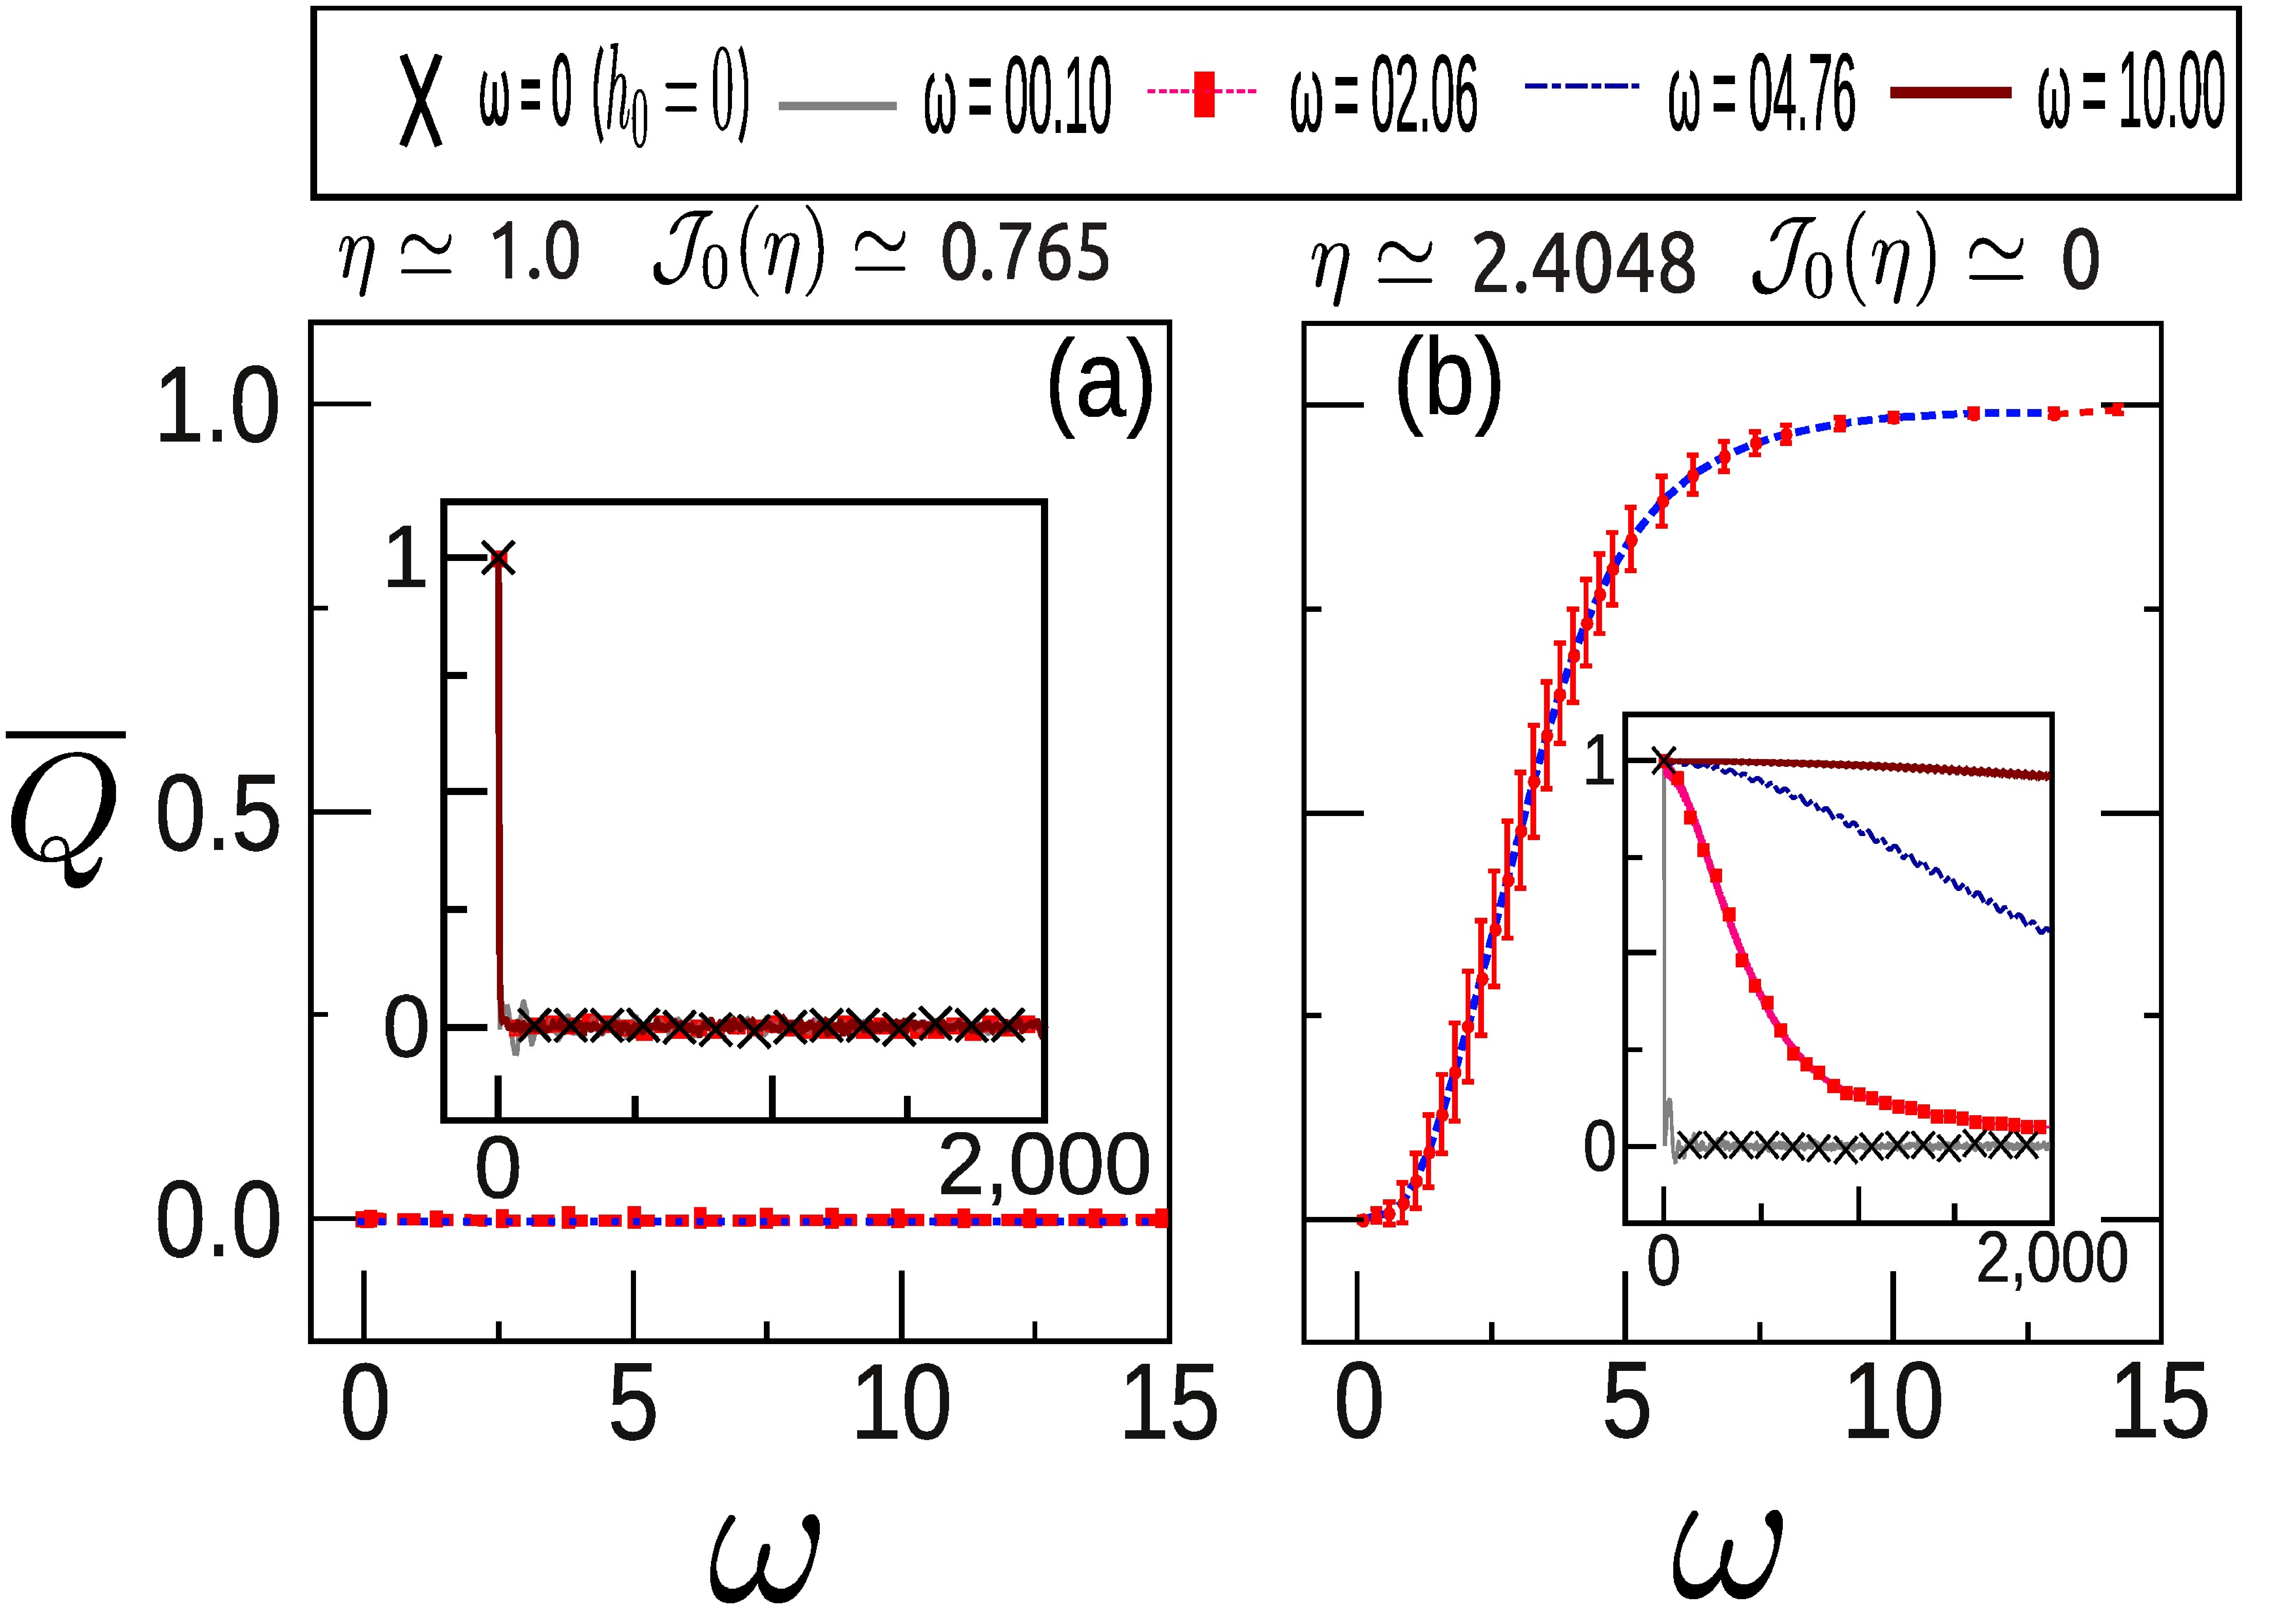
\epsfig{file=supp_fig1_hires.eps,height=2.75in,width=4.0in}
\caption{(Color Online) 
{\bf Disorder fluctuations in the numerics: Nonfreezing (a) vs Freezing (b)}:
{\bf (a)} Disorder average of magnetization (\textit{i.e.}  $\overline{Q}$ where  $Q\equiv\langle m^z(t)\rangle$), as well as fluctuations
(\textit{i.e.} $(\overline{Q^2}-\overline{Q}^2)^{1/2}$) as a function of $\omega$ (main-frame) with $h_0$ adjusted to keep $\eta\equiv 4h_0/\omega=1.0$, away from the freezing condition \textit{i.e.} $J_0(\eta) \ne 0$; {\bf inset} shows $\overline{m^{z}}$ vs $t$ - for corresponding cases. {\bf(b)} Under the freezing condition, $J_0(\eta) \approx 0$ at the first zero of the Bessel function. Here, $\overline{Q}$ approaches unity with increasing $\omega$ as predicted by the theory - the effective Hamiltonian (Eqs. \ref{eq:heff}) vanishes to order higher than one in $1/\omega$. In all plots, the field disorder is absent ($h_i=0$), $\hbar=1$, $J=1$, and the disorder strength $\alpha = 0.3$. The red error bars represent disorder fluctuations, and are negligible away from freezing (panel(a)), as well as at freezing for large $\omega$. The largest fluctuations occur when the freezing condition breaks down due to the contributions of higher order terms in the effective Hamiltonian, but do not go above $0.14$ as seen 
in panel (b).}
\label{fig:errbars}
\end{figure}

\section{\sc Analytical Treatment via unitary renormalization group flow in Floquet Space}
In this section, we elaborate on our analytical treatment of this problem by mapping the $T=2\pi/\omega$ - periodic Hamiltonian in the Hilbert space $\mathcal{H}$ to an effective time-independent Hamiltonian $H_{\rm eff}$ such that the unitary evolution coincides with $e^{i H_{\rm eff}\;t}$ when $t=nT$. In order to achieve this, we conceive a family of Hamiltonians $H(l;t)$, parametrized by $l$, all of which are linked to each other by unitary transformations given by the operation $P_{\;l_1,l_2;t}$, \textit{i.e.}  
\begin{equation}
H(l';t) = P_{\;l',l;t}\left[H(l;t)\right] \equiv Z^\dagger(l',l;t) H(l;t) Z(l',l;t) - i\; Z^\dagger(l',l;t) \bigg\{ \frac{\partial}{\partial t}Z(l',l;t) \bigg\}\; \forall\; l,l' ,
\end{equation}
and $H(0;t)$ is our original Hamiltonian $H(t)$. In addition, we conceive a parameter value $\bar{l}$ such that 
$H_{\rm eff} \approx H(\bar{l};t)= P_{\;\bar{l},0;t}\left[H(t)\right]$ is approximately time independent. This leads to the relation
\begin{equation}
\label{eq:strobe}
U(t) \approx e^{-iH_{\rm eff}t}Z(t)
\end{equation}
where we have dropped the dependencies on $\bar{l},l$, and $U(t)$ solves the Schr\"odinger equation for the original Hamiltonian \textit{viz.} $i\partial_t U(t) = H(t) U(t)$. Note that Floquet's theorem ensures (see~\cite{Analabha1,Analabha2} and references therein) that $Z(t)$ is time-periodic if $H(\bar{l};t)$ is time independent. If the family of transformations can be generated in such a way that $U(\bar{l},l;0)=\mathds{1}$, then this result can be combined with Eq.~\ref{eq:strobe} to yield $U(t)\approx e^{-iH_{\rm eff}t}$ at integer multiples of the period. Thus, the claim made in the main paper that $H_{\rm eff}$ is \textit{dynamically equivalent} to $H(t)$ when strobed at multiples of the time period is verified. The Wilson (Wegner) numerical renormalization group provides a systematic approach towards determining such a family of transformations, as well as the value $\bar{l}$, via unitary flows~\cite{Kehrein-book}. The three step prescription restricts such flows to the Floquet-Hilbert space that is 
appropriate for time-periodic Hamiltonians, and is detailed below.

The first of the three-step process, rewriting the spin Hamiltonian in bosonic language, has already been performed in Eq.~\ref{H_Fermi:suppl}. In the next step, we separate the Hamiltonian in Eq.~\ref{H_Fermi:suppl} into
$H(t) = H_s + H_d(t)$, where 
\begin{eqnarray} 
\label{eq:hshd}
H_s(J_i,h_i) &=& - \alpha J \sum_i^{L-1} J_i \left(c^{\dagger}_i c^{\dagger}_{i+1} + c^{\dagger}_i c_{i+1}  + {\rm h.c.}\right) 
    - 2 \alpha \sum_i^{L}  h_i c^{\dagger}_i c_i \; ,\nonumber \\
 H_d(J_i,t) &=& -2\; h(t)\sum_i^{L-1} c^{\dagger}_i c_i \; ,
\end{eqnarray}
This Hamiltonian is defined in a complete Hilbert space $\mathcal{H}$. In this Hilbert space, we transform the Hamiltonian by the unitary transformation $\Lambda(t) = \exp{\left\{i \int^t_0 \mathrm{d}\tau \; H_d(\tau)\right\}}$, yielding
\begin{eqnarray}
 \label{eq:htilde}
 \tilde{H}(t) &=& \Lambda(t)\; H(t)\; \Lambda^\dagger(t) - i \; \Lambda(t)\; \left\{\frac{\partial}{\partial t} \Lambda(t)\right\}^\dagger \nonumber \\
              &=& \Lambda(t)\; H_s\; \Lambda^\dagger(t).
\end{eqnarray}
This Hamiltonian, like the previous one, is periodic in time with period $T$. In that case, Floquet's theorem states that the corresponding Schr\"odinger equation can be solved by states of the type $|\psi_p (t) \rangle = e^{i \Omega_p t}\; |\phi_p(t)\rangle$, where $|\phi_p(t+nT)\rangle=|\phi_p(t)\rangle$, and the Floquet quasienergies $\Omega_p$ are real. Using Fourier's theorem, the Floquet eigenstates $|\phi_p(t)\rangle$ can be expanded in a basis $|n\rangle$, where $\langle t |n\rangle = e^{-i \; n\omega t}$. These basis states span a Hilbert space  $\mathcal{H}_T\subset \mathcal{H}$, consisting of states that are time-periodic in $T$, yielding $\tilde{H}(t) = \sum_n \tilde{H}_n\; e^{-i \; n\omega t}$, with
time-independent operators $\tilde{H}_n$. The corresponding Floquet operator $K(t)\equiv \tilde{H}(t)-i \;\partial_t$ is now mapped to an analogous operator $\mathcal{K}$ in the Floquet - Hilbert space  $\mathcal{H}\otimes\mathcal{H}_T$ to yield
\begin{equation}
\label{eq:floquetop:orig}
\mathcal{K} = \tilde{H}_0 \otimes \mathds{1} + \mathds{1}\otimes \omega \; \hat{n}  + \sum_{n\neq 0} \tilde{H}_n  \otimes \sigma_n.
\end{equation}
In Eq.~\ref{eq:floquetop:orig}, the operator $i \; \partial_t  $ has been mapped to $\mathds{1}\;\otimes\; \omega\; \hat{n}$. Here, the Floquet number operator acts only in $\mathcal{H}_T$ via the basis states as  $\hat{n} \; |n \rangle = n \;|n \rangle$. In addition, the operators $\sigma_n \in \mathcal{H}_T$ act as ladder operators on the basis states with $\sigma_m \; |n \rangle = |n +m\rangle$. Note that $\sigma_0 = \mathds{1}$, and the $n=0$ term in the structure of $\mathcal{K}$ is shown separately in Eq.~\ref{eq:floquetop:orig}. Starting from Eq.s~\ref{eq:htilde} and~\ref{eq:hshd}, as well as the Fourier expansion above, we can obtain the components $\tilde{H}_n$. Using the Jacobi-Anger expansion~\cite{watson}, $\exp{\left[i \; \eta \; \sin{\omega t}\right]}=\sum_m \mathcal{J}_m(\eta)\; e^{-i n \omega t}$, we obtain
\begin{equation}
\label{eq:h0}
\tilde{H}_0  =    -\alpha J\;\sum_{i=1}^{L-1} \mathcal{J}_0(\eta) J_i \left( c^\dagger_i c^\dagger_{i+1} + 						c^\dagger_i c^{\;}_{i+1} + \rm{h.c} \right) -2 \;\alpha\;\sum_{i=1}^{L-1} h_i c^\dagger_i c^{\;}_i,
\end{equation}
with $\eta\equiv4\; h_0/\omega$, and the $n\neq 0$ components given by $\tilde{H}_n   =    \sum_{i}  \tilde{H}^{(i)}_n$, where
\begin{equation}
\label{eq:hn}
\tilde{H}^{(i)}_n   \equiv -\alpha J J_i \bigg\{ \mathcal{J}_n(\eta)  \left( c^\dagger_i 		    c^\dagger_{i+1} + 					c^\dagger_i c^{\;}_{i+1} \right) +\mathcal{J}_{-n}(\eta) \left(c^{\;}_{i+1}c^{\;}_i + 		     						c^\dagger_{i+1} c^{\;}_{i} \right)\bigg\}.
\end{equation}
The ultimate purpose of writing our Hamiltonian in this manner is to use a systematic approach to renormalize the hopping terms in $\tilde{H}^{(i)}_n $ to determine any regime in the parameter space where they all might be ignored. The final step \textit{viz.}
the execution of this approach is described below.

The final step involves determining unitary transformations in $\mathcal{K}$ that lead to a dynamically equivalent expression whose time dependent parts ($\tilde{H}_{n\neq0}$) vanish, yielding an effective Hamiltonian $H_{\rm eff} = \tilde{H}_0$. In order to do so, we insert an unknown parameter $l$ and seek a family of unitary transformations on $\mathcal{K}(l)\in\mathcal{H}\otimes\mathcal{H}_T $ generated by choosing antihermitian operators $\Gamma(l)\in\mathcal{H}\otimes\mathcal{H}_T$, such that $\mathcal{K} = \mathcal{K}(l)|_{l=0}$, and the flow equations,
\begin{equation}
\label{eq:flows}
\frac{\mathrm{d}}{\mathrm{d}l}\;\mathcal{K}(l) = \bigg[\Gamma(l)\;,\;\mathcal{K}(l)\bigg],
\end{equation}
are satisfied by all $\mathcal{K}(l)$ while maintaining the same component structure as shown in Eq.~\ref{eq:floquetop:orig}. This way, our theory remains 'renormalizable' for all $l$. Any terms that do not belong in one of the components are 'non-renormalizable', and are reduced iteratively by generating new trials for $\Gamma(l)$ that absorb these terms. The fixed point of Eq.~\ref{eq:flows} (at, say $l=\bar{l}$) should yield the time-independent Hamiltonian via the solution $U^\dagger_s(\bar{l},t) H_{\rm eff} U_s(\bar{l},t)$, where $U_s(l,t)$ are the unitary transformations that link the different $\mathcal{K}(l)$ to $\mathcal{K}(0)$. In order to obtain the first iterative solution for Eq.~\ref{eq:flows}, we choose for $\Gamma(l)$ the Wilson generator~\cite{Wilson,Glazek,Mintert} 
\begin{equation}
\label{eq:g1}
\Gamma_1(l) = \sum_{n\neq 0} b_n(l) \left[\mathds{1}\otimes\omega \hat{n}, \tilde{H}_n \otimes  \left(\sigma_n-\mathds{1}\right) \right],
\end{equation}
and the trial solution for the corresponding flow in Eq.~\ref{eq:flows},
\begin{equation}
\label{eq:k1}
\mathcal{K}_1(l) = \tilde{H}_0 \otimes \mathds{1} + \mathds{1}\otimes \omega \; \hat{n}  + \sum_{j, m\neq 0}  b_m(l)\;\tilde{H}_m(J_j)  \otimes \sigma_m,
\end{equation}
with the initial condition $b_m(0)=1$. In Eq. \ref{eq:g1}, the RHS is the commutator between the only term in $\mathcal{K}(l)$ that is fully diagonal in $\mathcal{H}\otimes\mathcal{H}_T$~\cite{Glazek}, and the time-dependent parts of $\mathcal{K}(l)$ that come from the nonzero Fourier modes of $\tilde{H}(t)$. The choice of $\left(\sigma_n-\mathds{1}\right)$ over $\sigma_n$ in Eq.~\ref{eq:g1} ensures that the unitary transformation that takes $H(t)$ to $H_{\rm eff}$ is unity at $t=0$~\cite{Mintert}. Substituting Eqs.~\ref{eq:k1} and~\ref{eq:g1} into Eq.~\ref{eq:flows} yields a dynamical system after comparing terms on both sides, $b'_n(l)=-\omega^2 n^2 b_n(l)$, or $b_n(l)=\exp{\left(-n^2\omega^2 l\right)}$. Here, we have dropped all  non-renormalizable terms in the RHS of Eq.~\ref{eq:flows}. These are now sent to the next iteration, which yields the dominant contribution in $\omega$. The new generator, chosen in a manner similar to the previous iteration, is
\begin{eqnarray}
\label{eq:g2}
\Gamma_2( l) &=& \Gamma_1( l)+ {2\alpha^2 J}\sum_{i,n\neq0}   b_n(l)\; J_i\; h_i 
\bigg\{\mathcal{J}_n(\eta)\hat{f}^{\dagger}_i- \mathcal{J}_{-n}(\eta)\hat{f}^{\;}_i   \bigg\}\otimes \left(\sigma_n-\mathds{1}\right),\nonumber \\
\hat{f}^{\dagger}_i &\equiv& c^\dagger_{i-1}\left(c^{\;}_i - c^\dagger_i\right) - c^\dagger_i\left( c^\dagger_{i+1}+c^{\;}_{i+1} \right).
\end{eqnarray}
Analogously, the trial for the next iteration is
\begin{equation}
\label{eq:k2}
\mathcal{K}_2( l) = \mathcal{K}_1( l)+\alpha\sum_{i}  J_i\; h_i \bigg\{a_+(l)\hat{f}^\dagger_i -
a_-(l)\hat{f}^{\;}_i\bigg\}\otimes \mathds{1},
\end{equation}
with new parameters $a_\pm(l)$, and the initial conditions $a_\pm(0)=0\;,\;b_m(0)=1$ keep $\mathcal{K}(0)=\mathcal{K}$. Substituting these into Eq.~\ref{eq:flows} and comparing like terms on both sides yields the following nontrivial flow dynamics for the parameters, 
\begin{eqnarray}
\label{eq:rgflow}
 \frac{\mathrm{d}b_n}{\mathrm{d}l} &=& -\omega^2 n^2 b_n, \nonumber \\
 \frac{\mathrm{d}a_+}{\mathrm{d}l} &=& -2\alpha J \omega \sum_{n\neq0} n b_{n}(l)\; \mathcal{J}_n(\eta),\nonumber \\
 \frac{\mathrm{d}a_-}{\mathrm{d}l} &=& +2\alpha J \omega \sum_{n\neq0} n b_{-n}(l) \; \mathcal{J}_n(\eta),
\end{eqnarray}
where we have truncated out non-renormalizable terms 
\footnote{The largest non-renormalizable term leftover in $\left[\Gamma_2(l),\mathcal{K}_2(l)\right]$ is $$\left[\Gamma_1(l), \mathcal{K}_2(l)-\mathcal{K}_1(l) \right] =\alpha J \omega^2 \sum_{i,j,n\neq 0} n b_n(l) J_i h_i \left[H_n^{(j)},a_+(l)f^\dagger_i-a_-(l)f^{\;}_i\right] \otimes \left(\sigma_n-\mathds{1}\right).$$ Substituting the value of $H^{(j)}_n$ from eqn.~\ref{eq:hn} yields contributions that go as $J_i J_j$ , with no like terms in the $l$-derivative of the trial $\mathcal{K}_2(l)$​ ​in eqn.~\ref{eq:k2} ​with which to compare. However, given that  $|J_i|<1$, these terms can be ignored in comparison to dominant contributions that are linear in $J_i$ . In order to obtain their effects, the next trial for $\mathcal{K}(l)$, as well as corresponding choice for $\Gamma(l)$, will have to absorb them with a new set of flow parameters as weights. The other leftover term is $\left[\Gamma_2(l)-\Gamma_1(l),\mathcal{K}_2(l)-\mathcal{K}_1(l)\right]$, which goes as $\alpha^3$ and can be ignored for small 
disorder strength.}
by substituting $a_\pm(l)=a\pm(0)=0$ on the RHS of the flow equation for this iteration~\cite{Mintert}. These equations yield the same solution for $b_n$ as the previous iteration, and
\begin{equation}
a_\pm(l) = \mp\frac{2\alpha J}{\omega}  \sum_{n\neq0} \left(1-e^{-n^2\omega^2 l}\right)\; \frac{\mathcal{J}_n(\eta)}{n}.
\end{equation}
The fixed point of the flow dynamics occurs when $l\rightarrow\infty$, where $a_\pm(\infty)=\mp {2\alpha J\beta(\eta)}/{\omega}$, and $\beta(\eta)\equiv\sum_{n\neq 0} {\mathcal{J}_n(\eta)}/{n}$. Substituting these in Eqs.~\ref{eq:k2} and~\ref{eq:k1} yields
\begin{equation}
\label{eq:floquetop}
\mathcal{K}_2(\infty) =  \bigg\{\tilde{H}_0-\frac{2\alpha^2 J}{\omega}\;\beta(\eta)\sum_{i}  J_i h_i \left(\hat{f}^{\;}_i + \hat{f}^\dagger_i\right)\bigg\}\otimes \mathds{1} 
+\mathds{1}\;\otimes \; \omega \hat{n} + \mathcal{O}(\alpha/\omega^2).
\end{equation}
In Eq.~\ref{eq:floquetop}, we identify the first part in the sum on the RHS with the time-independent part of the Hamiltonian, $\tilde{H}_0 \in \mathcal{H}$, the second part with the operator $-i \; \partial_t  \in \mathcal{H}_T$, and all the $\tilde{H}_{n\neq 0}$  as the time-dependent parts, which scale as $\mathcal{O}(\omega^{-2})$. Thus, this new Floquet operator maps to a time-independent Hamiltonian $H_{\rm eff}\in\mathcal{H}$ up to $\mathcal{O}(\omega^{-1})$, \textit{viz.}
\begin{eqnarray}
\label{eq:heff}
H_{\rm eff}    &=&   -J\sum_i j^{(0)}_i\left(c^\dagger_i c^\dagger_{i+1} + \rm{h.c.}\right) 
		            -J\sum_i j^{(1)}_i\left(c^\dagger_i c^{\;}_{i+1}+\rm{h.c}\right) 
		            -\mu\sum_i j^{(2)}_i c^\dagger_i c^{\;}_i, \nonumber \\
j^{(0)}_i            &\equiv& \alpha J_i\; \bigg\{\mathcal{J}_0(\eta) - \frac{4\alpha h_i}{\omega}\beta(\eta)\bigg\} ,\nonumber \\
j^{(1)}_i            &\equiv& \alpha J_i \; \mathcal{J}_0(\eta) ,\nonumber \\
j^{(2)}_i            &\equiv& \frac{h_i}{J},\nonumber \\
\mu 		     &\equiv& 2\alpha J.
\end{eqnarray}
Note that, in order to obtain $H_{\rm eff}$, we have canceled out terms like $\sum_i c^\dagger_{i-1}c^{\;}_i$ with terms like $\sum_i c^\dagger_i c^{\;}_{i+1}$ while summing over large number of lattice indices. Setting the field disorder $h_i$ to zero recovers the analytical results discussed in the main paper, where the full Hamiltonian maps via unitary flows to an \textit{identical} effective Hamiltonian with renormalized hopping $J\rightarrow J \mathcal{J}_0(\eta)$.
%%%%%%%%%%%%%%%%%%%%%%%%%%%%%%%%%%%%%%%%%%%%%%%%%%%%%%%%%%%%%%%%%%%%%%%%%%%%%%%%%%%%%%%%%%	
%Note: Change 'highres' to 'lowres' in figs for arxiv submission
%%%%%%%%%%%%%%%%%%%%%%%%%%%%%%%%%%%%%%%%%%%%%%%%%%%%%%%%%%%%%%%%%%%%%%%%%%%%%%%%%%%%%%%%%%
 \begin{figure}[!t]
 \ 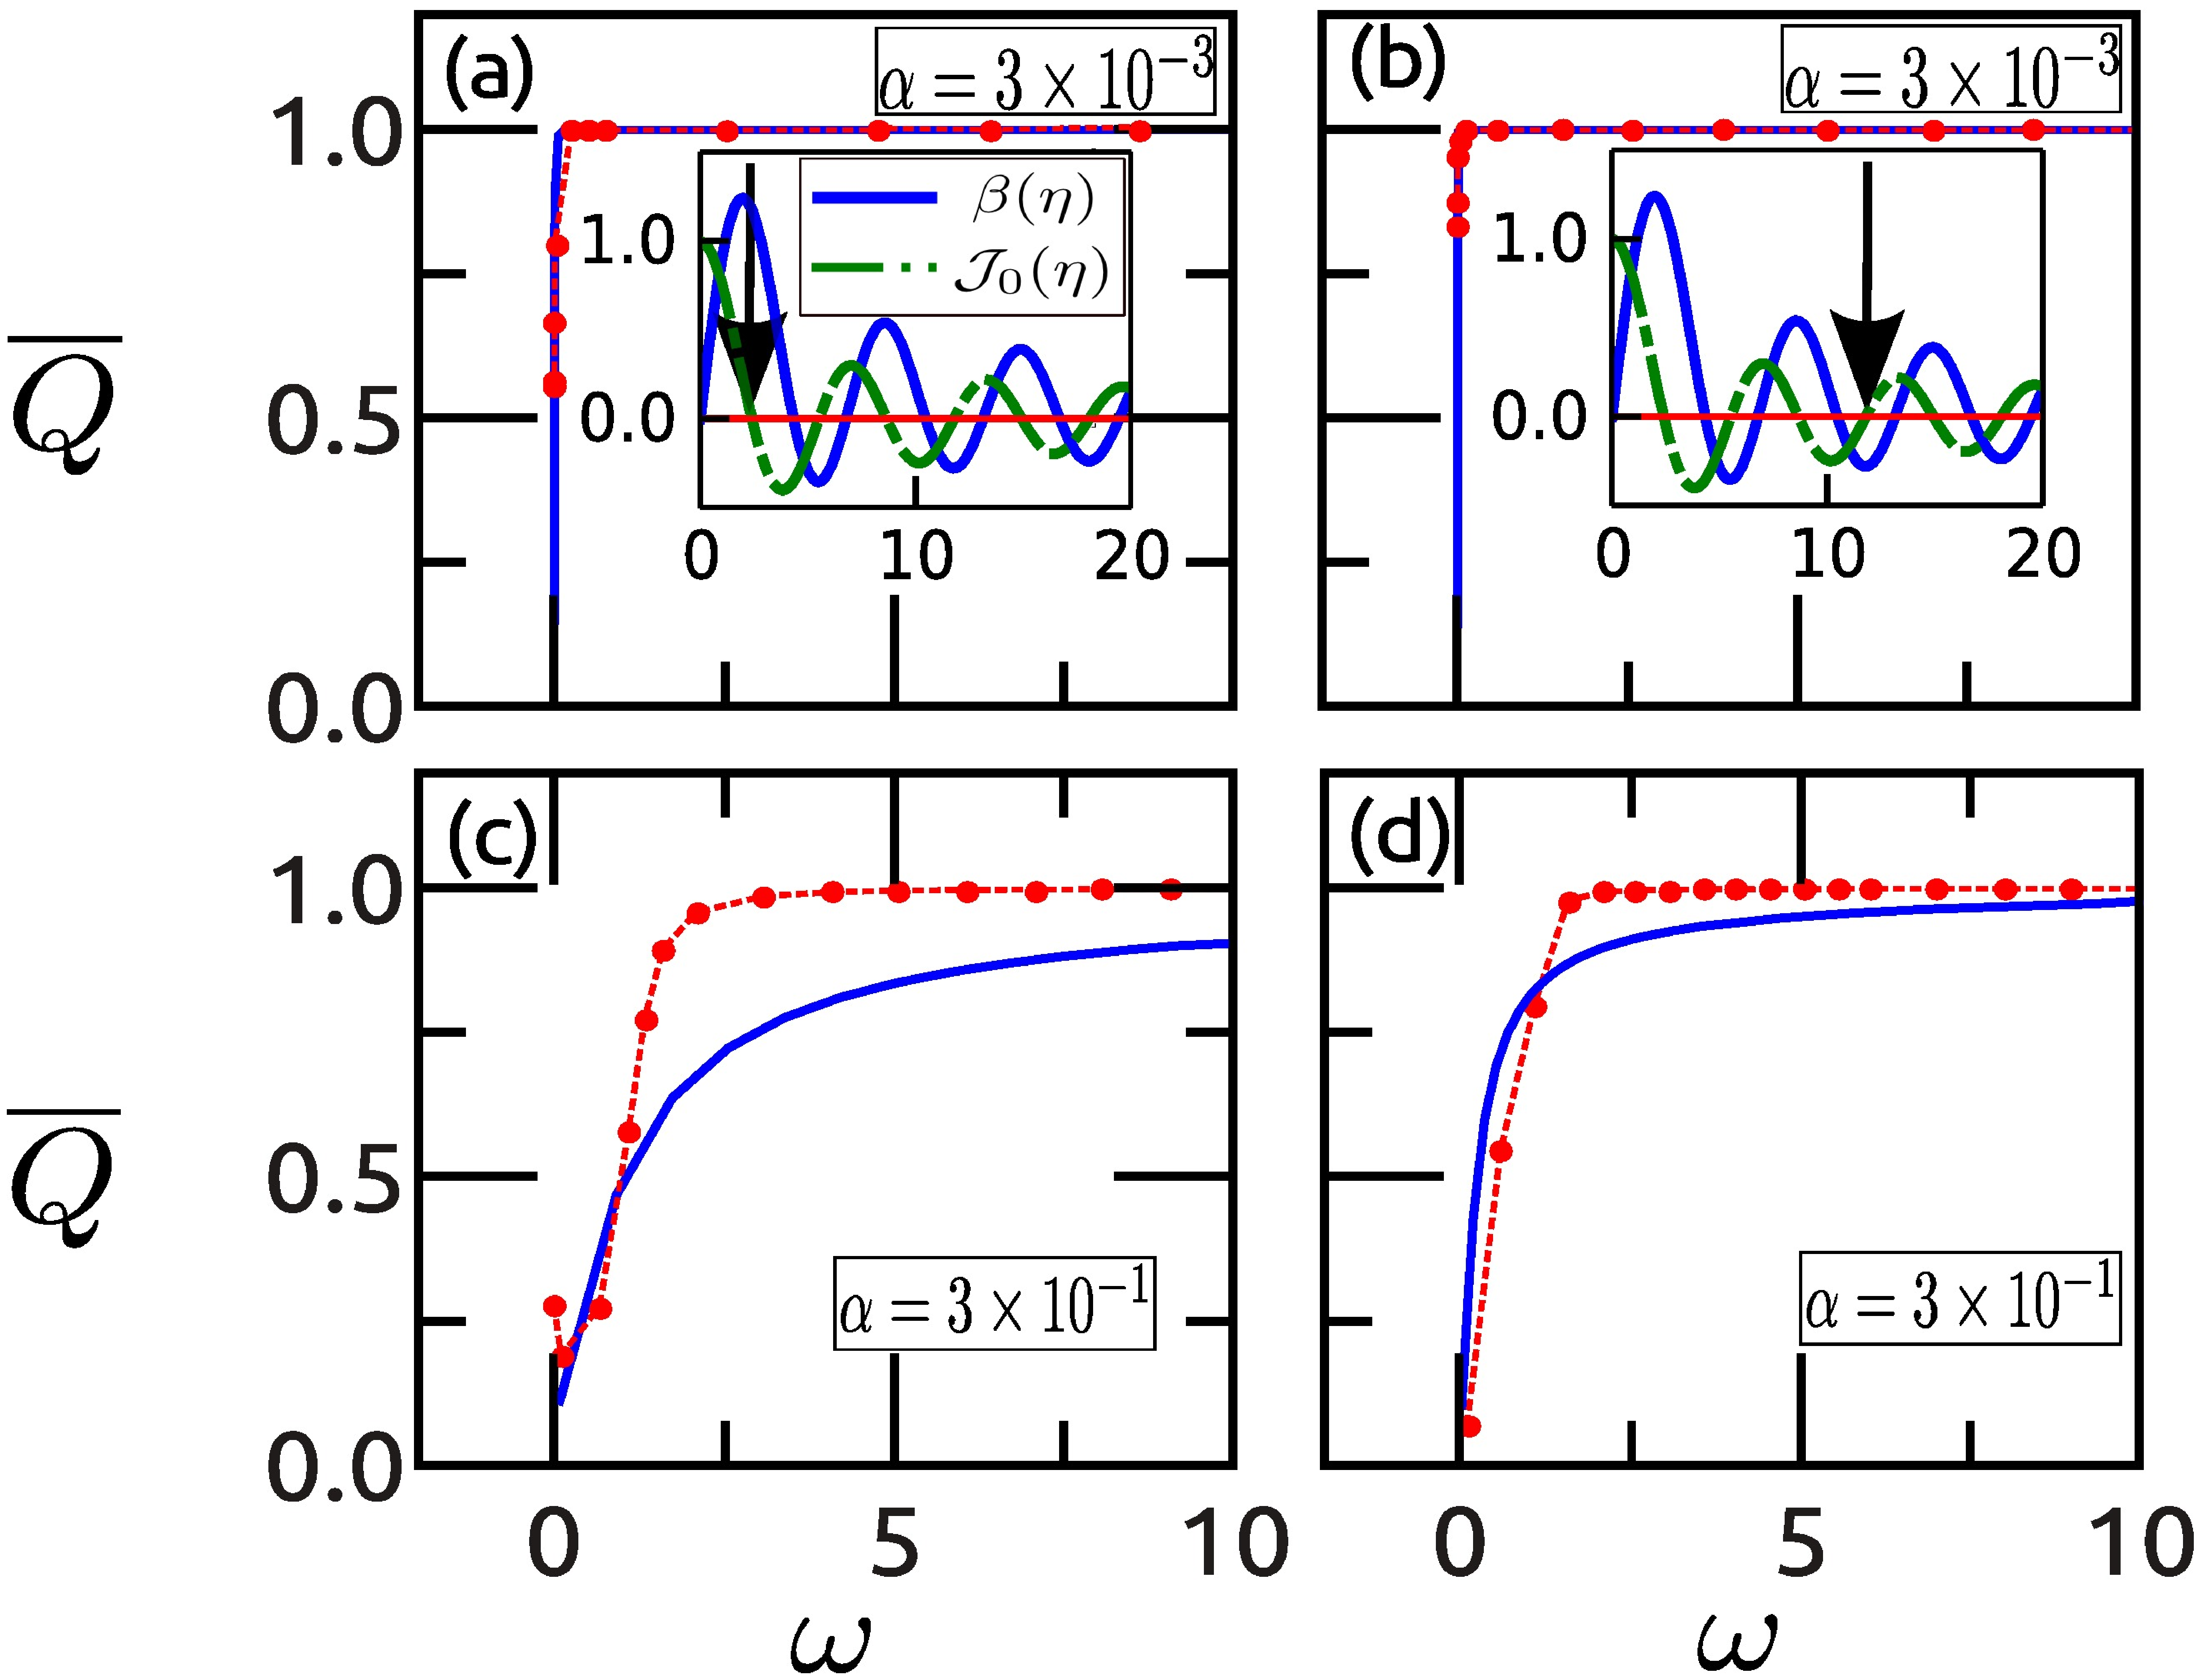
\epsfig{file=supp_fig2_hires.eps,height=2.75in,width=3.3in}
 \caption{(Color Online) Plots of $\overline{Q} $ \textit{v.s.} $\omega$ for two different values of $\alpha$. In the main panels, the red circles  (blue curves) plot the ordinate obtained from the time-evolution of the full Hamiltonian given by Eq.~\ref{H_Fermi:suppl} (effective Hamiltonian given by Eqs. \ref{eq:heff}) averaged over $t=\left[0,300\right]$, and $10^3$ disorder realizations. The values of $\alpha$ chosen are indicated in the main legends. Panels {\bf (a)} and {\bf (c)}: The value of $\eta=4h_0/\omega$ was kept fixed at the first root of $\mathcal{J}_0(\eta)$ as indicated by a gray arrow next to the plot of $\mathcal{J}_0$ (green dashed) in the inset on panel (a). Panels {\bf (b)} and {\bf (d)}: Here, $\eta$ was fixed at the fourth root as indicated in the inset on panel (b). In both insets, the blue curves  plot $\beta(\eta)$.}
 \label{fig:multw:qcomp}
 \end{figure}
 
\section{\sc Comparison with numerics}

The validity and limits of our theoretical description in the previous section can be quantitatively determined by evolving the dynamics in 
Eq.~\ref{BdG_tdep:eqn} in the first section with the time-independent $H_{\rm eff}$ in Eq.~\ref{eq:heff}. 
Switching to the fermion representation leaves the $H_{\rm eff}$ invariant, and the matrices $A(t), B(t)$ 
are time independent. The nonzero matrix elements in the dynamics for $H_{\rm eff}$ are given by
$A_{ij} = -\alpha h_i \; \delta_{ij}$, $B_{i,i+1}=-B_{i+1,i} = \alpha J j_i/2$ at any freezing 
point given by $\mathcal{J}_0(\eta)=0$. The quantities $\overline{Q}$ and $\overline{m^{z}(t)}$ 
can be extracted and compared with those from the evolution of Eq.~\ref{BdG_tdep:eqn} with 
the full Hamiltonian in Eq.~\ref{H_Fermi:suppl}. Figure~\ref{fig:multw:qcomp} shows plots comparing the approach to 
freezing in $\overline{Q}$ with increasing $\omega$ for both the time evolution of $H(t)$ and $H_{\rm eff}$. 
The left panels show plots when $h_0$ is adjusted for each $\omega$ such that $\eta$ is at the first 
root of the zeroth order Bessel function, and the right panels show similar plots for the fourth root. 
Based on the structure of our truncated approximation for $H_{\rm eff}$ in Eq.~\ref{eq:heff}, we expect 
that higher order contributions will be controlled by powers of the disorder strength $\alpha$, 
as well as the value of $\beta(\eta)$ at freezing. This is borne out by the data shown in Fig.~\ref{fig:multw:qcomp}. 
When $\eta$ is at the first root of $\mathcal{J}_0$, the value of $\beta(\eta)$ is near-maximum (see the insets of Fig.~\ref{fig:multw:qcomp}). Here, contributions from the higher order terms cause theory to differ from the numerics quantitatively if $\alpha$ is appreciable. This can be seen  in Fig~\ref{fig:multw:qcomp} (c), where $\alpha=0.3$. However, these deviations are smaller 
when $\alpha$ is decreased to $0.003$ as seen in Fig~\ref{fig:multw:qcomp} (a). The function $\beta(\eta)$ decreases 
non-monotonically with increasing $\eta$ (insets in Fig~\ref{fig:multw:qcomp}), suppressing higher order contributions at 
larger roots. Note that  $\mathcal{J}_0(\eta)$ and $\beta(\eta)$ never vanish simultaneously. 
The best agreement is in Fig~\ref{fig:multw:qcomp} (b), where $\alpha$ and $\beta(\eta)$ are the smallest among the chosen values at freezing. 

Another aspect of the exact dynamics that can be inferred from the effective Hamiltonian in Eq.~\ref{eq:heff} is the time-scale of the magnetization at or near the roots of the function $\beta(\eta)$. If we switch off the field disorder $h_i$ by replacing them with a constant transverse field $h_i=J$, then, in the immediate neighborhood of a root of $\beta(\eta_r)$, a Taylor expansion yields $j^{(0)}_i \approx \alpha J_i\{ \mathcal{J}_0(\eta_r)-(4\alpha J/\omega) (\eta-\eta_r)\beta'(\eta_r)\}$, where $\beta'$ denotes the $\eta-$ derivative of $\beta$. Since $\eta$ and $\eta_r$ both scale inversely with $\omega$, varying $\eta$ by varying $h_0$ alone leads to a $\omega^{-2} - $ dependence on the second term, allowing us to ignore it for large $\omega$. Thus, the contribution of the transverse field at or near the roots of $\beta$ is 
%%%%%%%%%%%%%%%%%%%%%%%%%%%%%%%%%%%%%%%%%%%%%%%%%%%%%%%%%%%%%%%%%%%%%%%%%%%%%%%%%%%%%%%%%%	
%Note: Change 'highres' to 'lowres' in figs for arxiv submission
%%%%%%%%%%%%%%%%%%%%%%%%%%%%%%%%%%%%%%%%%%%%%%%%%%%%%%%%%%%%%%%%%%%%%%%%%%%%%%%%%%%%%%%%%%
\begin{figure}[!t]
\ \epsfig{file=supp_fig3_hires.eps,width=2.5in}
\caption{(Color Online) 
Here we plot $\tau$ vs $1/{\mathcal J}_{0}(\eta)$ for discrete values of $\eta$
for which $\beta(\eta)=0$ (six smallest roots) is satisfied. Plots for different values of $J$ are shown.  
We observe a linear behavior (discrete data points fitted with least-square lines) in the regime $\mu \ll J.$
This can be explained from the fact that for $\beta(\eta) = 0$ and $\mu \ll J$, $H_{eff} \propto {\mathcal J}_{0}(\eta)$
(Eq.~\ref{eq:heff}) to a good approximation, and hence all timescales (including) $\tau$ should be proportional 
to $1/{\mathcal J}_{0}(\eta)$. The inset shows continuous plots of $\tau$ vs $1/|\mathcal{J}_0(\eta)|$ in the 
immediate neighborhood of a root of $\beta(\eta)$. The root is indicated by a vertical (dot-dashed) red line, 
and the values of $J$ chosen are indicated in the main legend.
} 
\label{fig:tfield}
\end{figure}
negligible in this regime. In this regime, the time-scale $\tau$ of the magnetization $m^z(t)$ is expected to scale linearly with the inverse of the renormalized hopping \textit{viz.} $1/|J\mathcal{J}_0(\eta)|$ provided $J$ is sufficiently large compared to $\alpha$ so as to minimize the dynamical effects of the bond disorder. Figure~\ref{fig:tfield} shows plots of the time-scale $\tau$, obtained via exponential fit to the decay of $m^z(t)$, at the first six roots of $\beta(\eta)$. The data is plotted against $1/|\mathcal{J}_0(\eta)|$, and the points fitted by 
least-squares to lines. The plots demonstrate that the fits get progressively better as $J$ is increased, with deviations due to bond disorder becoming more and more prominent at smaller $J$. The inset also shows continuous plots of $\tau$ vs. $1/|\mathcal{J}_0(\eta)|$ in the immediate neighborhood of a single root of $\beta(\eta)$ (shown as a vertical red line), demonstrating approximately linear behavior in the vicinity of the root. Deviations from linearity occur for larger values of $\eta$, where higher order terms in the Taylor expansion begin to contribute. These contributions are non-monotonic, however, and reduce as $\eta$ approaches another root of $\beta$.
\afterpage{\clearpage}
\bibliographystyle{apsrev4-1}
\bibliography{bib_freezing}
\end{document}
